\chapter*{Aufgabe 1}
    Die Ticketagentur verkauft \textcolor{blue}{Eintrittskarten (Tickets)} für unterschiedliche Veranstaltungen. \textcolor{blue}{Veranstaltungen} haben
    einen \textcolor{blue}{Titel}, eine \textcolor{blue}{Beschreibung} und kennen \textcolor{blue}{Datum} und \textcolor{blue}{Ort} an dem sie stattfinden. Je nach Veranstaltung ist das
    \textcolor{blue}{Ticketkontingent} unterschiedlich groß. Veranstaltungen können im System auch ein leeres Ticketkontingent haben.
    Jedes Ticket hat einen \textcolor{blue}{Preis}, eine \textcolor{blue}{Ticketnummer} und ist für genau eine Veranstaltung gültig. Neben normalen
    Tickets gibt es \textcolor{blue}{Gruppentickets} und \textcolor{blue}{personalisierte Tickets}. Gruppentickets kennen die \textcolor{blue}{Anzahl der Personen}, die mit
    dem Ticket Zutritt zur Veranstaltung bekommen. Personalisierte Tickets sind genau je einer Person zugeordnet.
    Natürlich können verschiedene personalisierte Tickets, derselben Person zugeordnet sein. Personen haben einen
    \textcolor{blue}{Namen} und eine \textcolor{blue}{Adresse}.
    \textcolor{blue}{Käufer/innen} sind Personen und müssen im System registriert sein, um Tickets kaufen zu können. Von ihnen ist
    außerdem noch die \textcolor{blue}{Kreditkartennummer} bekannt. Käufer/innen können personalisierte Tickets auch für andere
    Personen (und nicht unbedingt nur für sich selber) kaufen.
    Die Ticketagentur bietet außerdem \textcolor{blue}{Veranstaltungskataloge} für unterschiedliche \textcolor{blue}{Genre} an. Ein solcher Katalog muss
    auf jeden Fall mehr als 10 Veranstaltungen enthalten. Jede Veranstaltung wird in mindestens einem Katalog gelistet.
    
    
    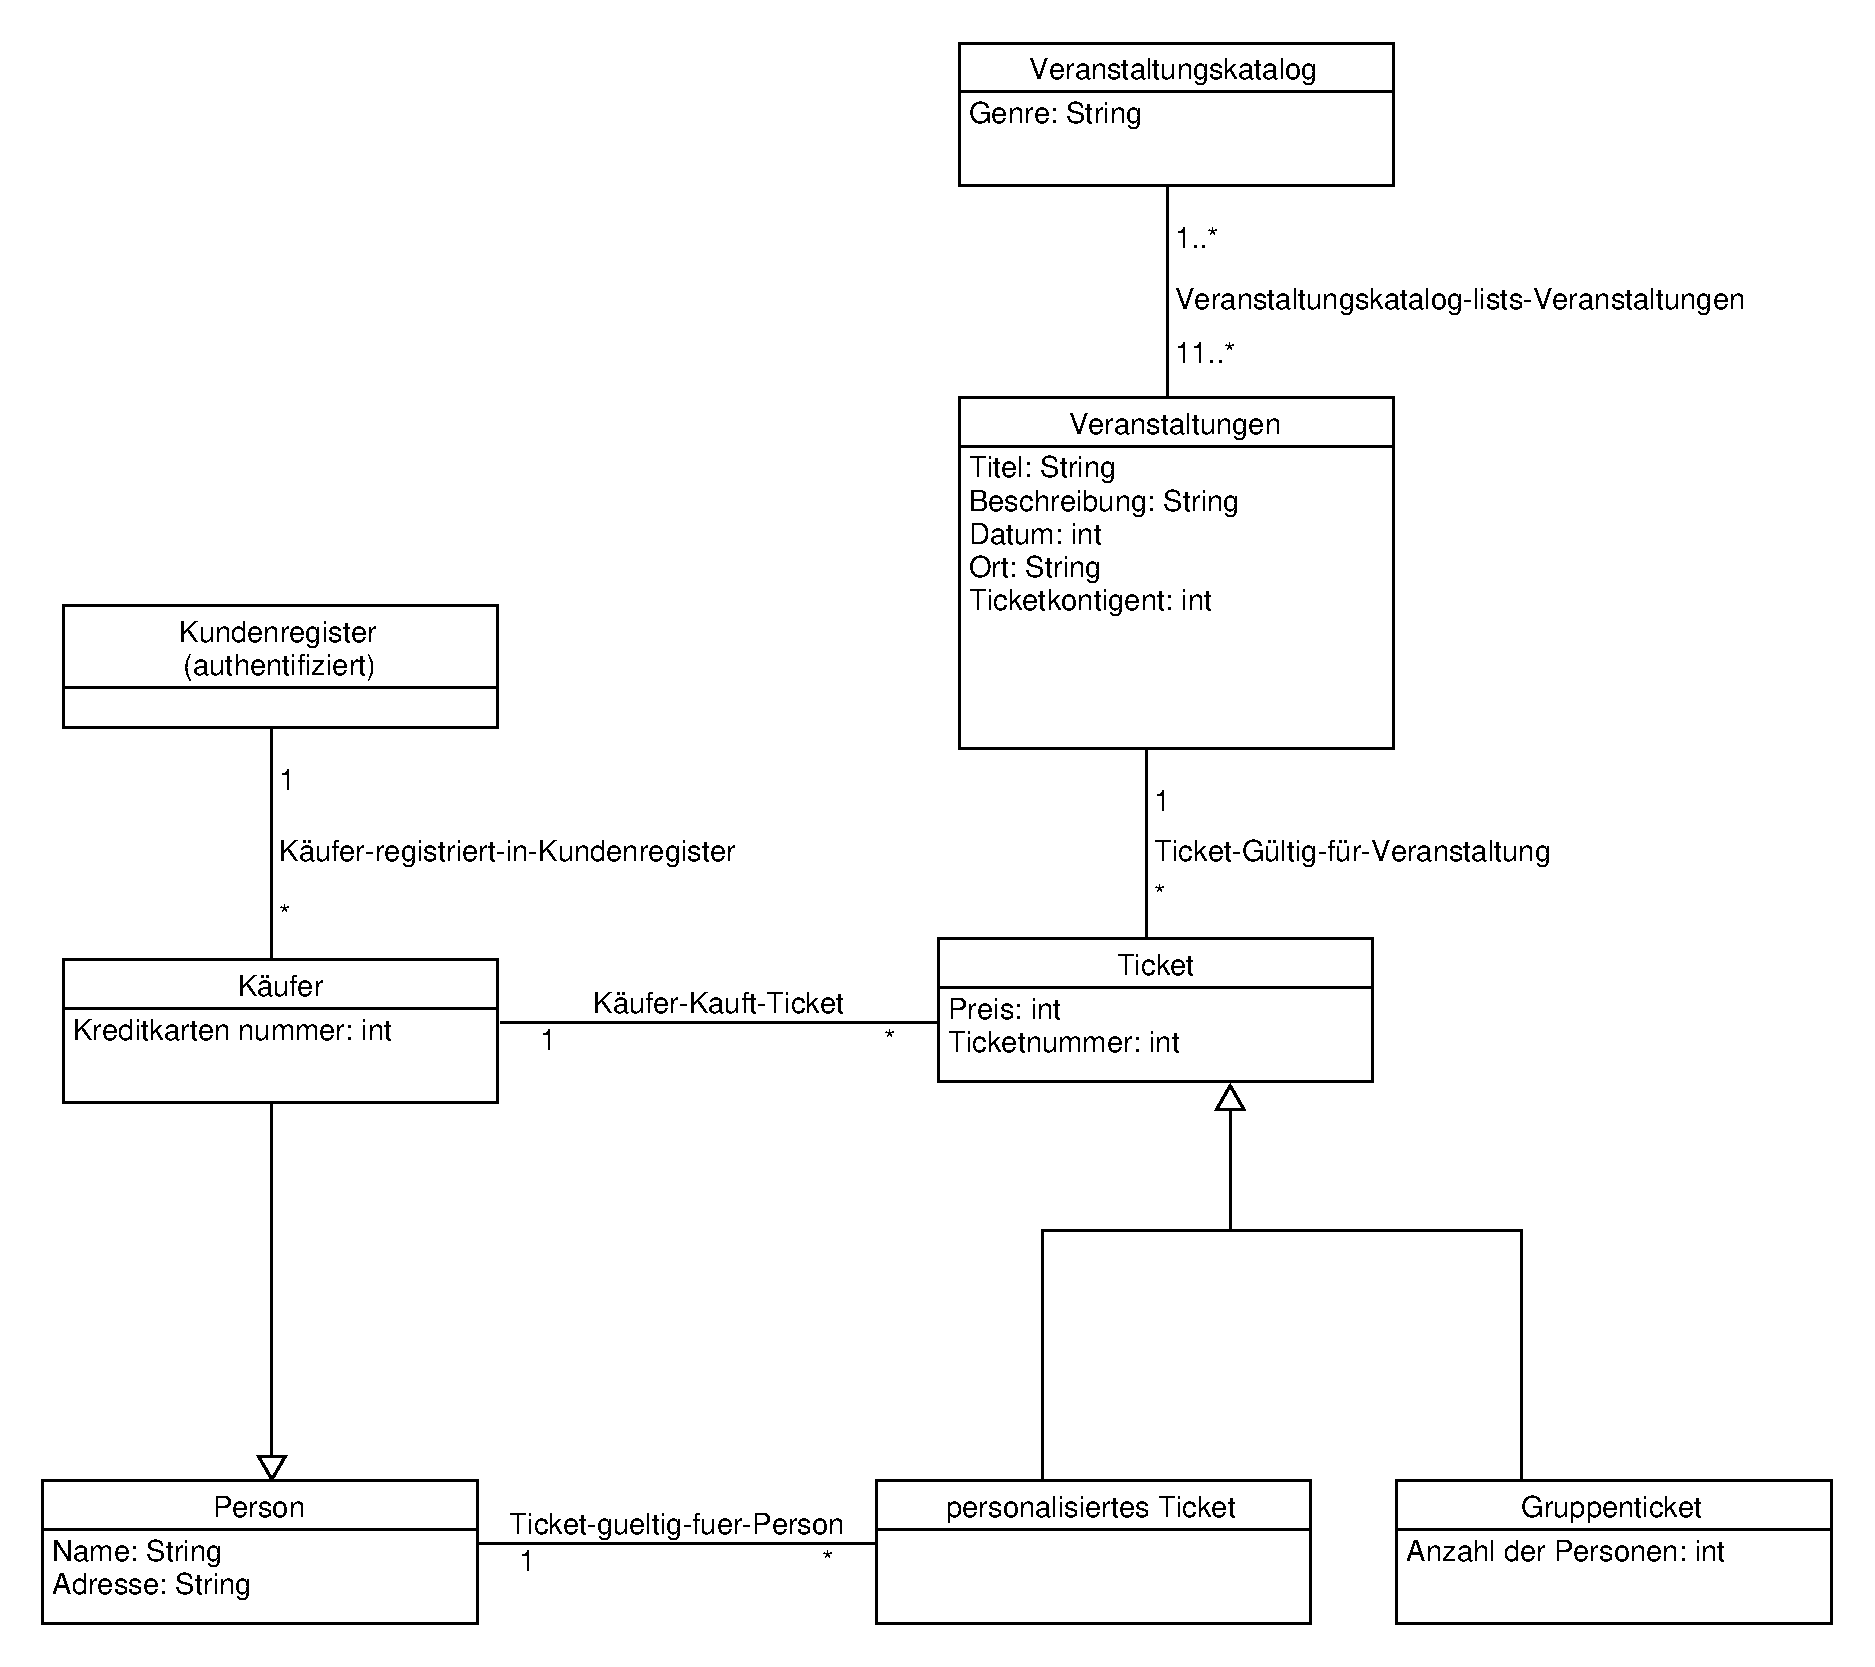
\includepdf{Visualisierungen/SEUe03UML.pdf}